\subsection{M.PD.14 - Complessità ciclomatica}

\begin{figure}[H]
  \centering
  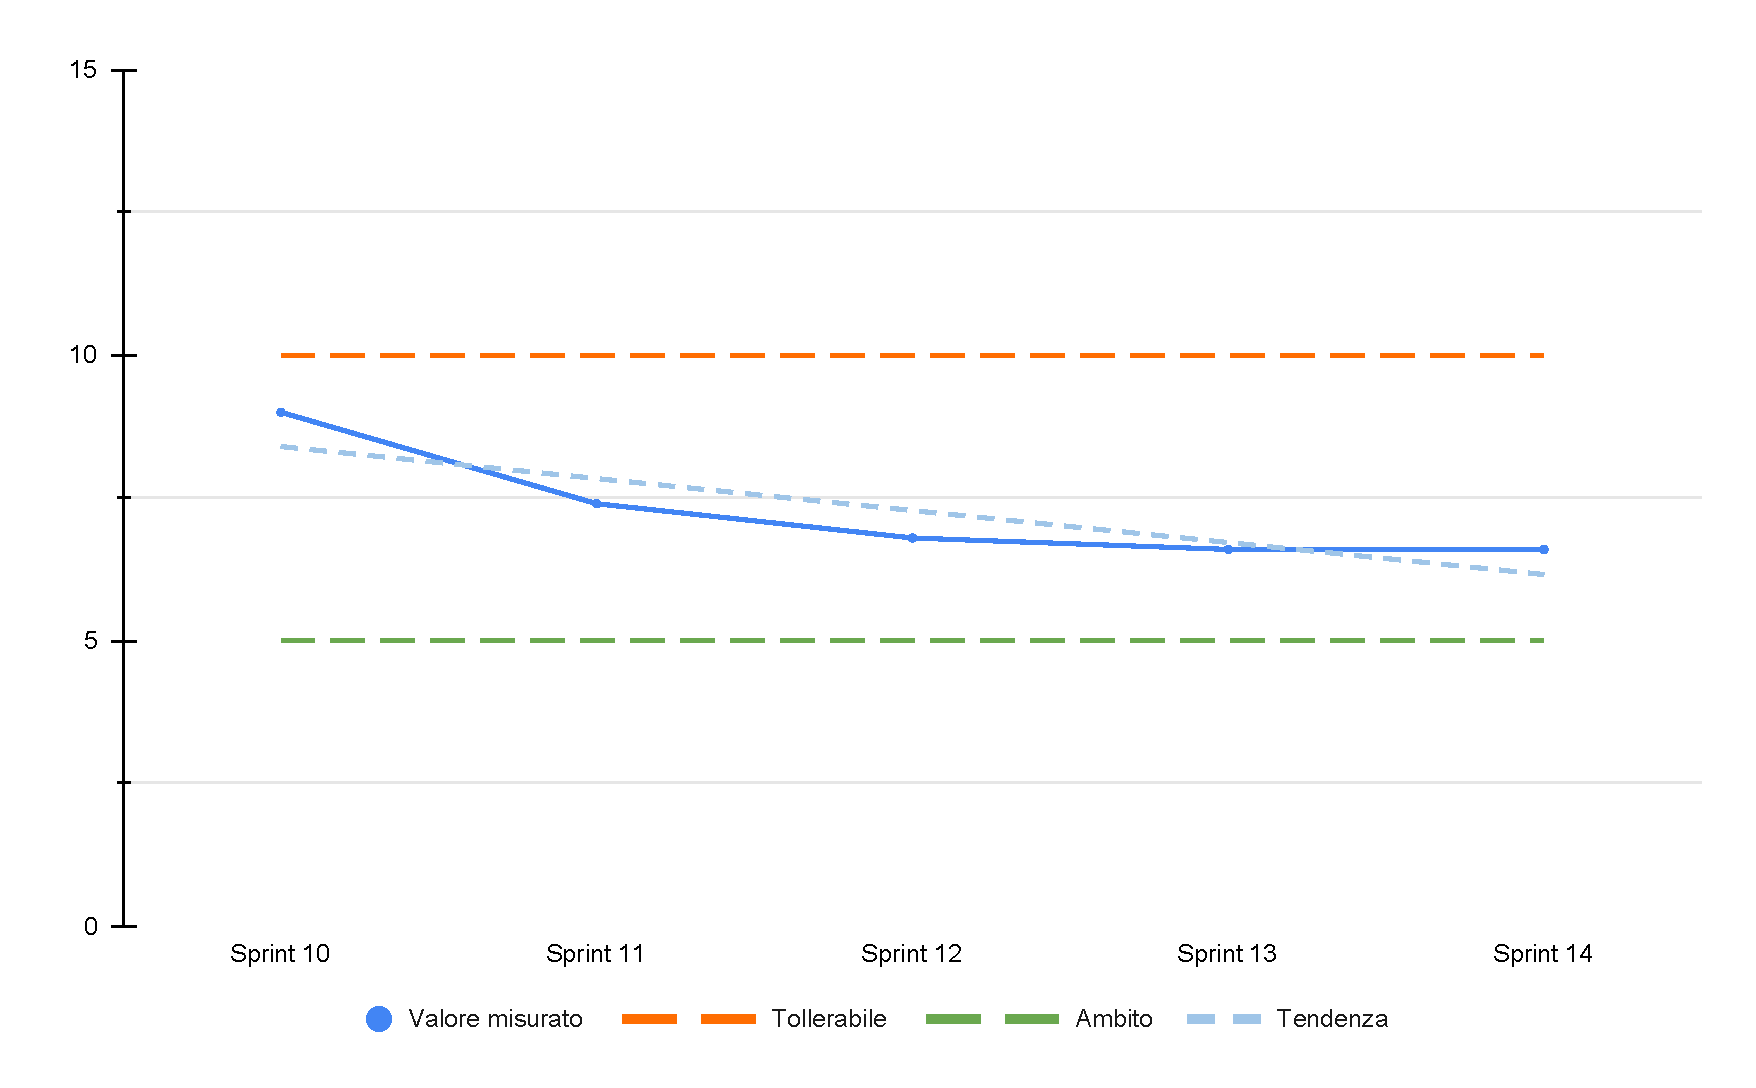
\includegraphics[width=\textwidth]{assets/complessita_ciclomatica.pdf}
  \caption{M.PD.14 - Complessità ciclomatica}
\end{figure}

\par La complessità ciclomatica è rimasta entro i limiti di tollerabilità per tutta la durata della \glossario{PB}. Il grafico evidenzia un picco di complessità in corrispondenza dello \glossario{sprint} 10, quando la progettazione era ancora in fase preliminare. Con l'avvio del refactoring e l'implementazione del modello architetturale selezionato, il gruppo ha osservato una diminuzione costante della complessità. Questo miglioramento è stato anche conseguenza della rielaborazione delle funzioni più complesse, che sono state suddivise in unità più piccole e con responsabilità limitate. Per quanto riguarda i test, il team è riuscito a mantenere la complessità ciclomatica inferiore a 10, rispettando il range previsto dal \PdQ.